\chapter[Kaggle]
{Kaggle}
\section{Regresión}
\section{Descripción del problema}
\subsection{Evaluación}
\section{Algoritmos}
\textbf{Nota: Para la ejecución de los algoritmos los datos nominales se han pasado a numérico}

A priori desconocemos que algoritmo se adapta mejor a nuestro problema, es por ello que realizaremos un estudio comparando varios algoritmos. Los algoritmos elegidos son los siguientes:
\begin{itemize}
	\item Un algoritmo clásico como la regresión lineal.
	\item Algoritmos "básicos" como KNN y Árboles de clasificación y regresión(CART).
	\item Otros algoritmos como NeuralNetwork,Gaussian y SVR(para hallar relaciones no lineales)
	\item Multiclasificadores ya que debido a su fácil paralelización ofrecen una buena escalabilidad. En este caso he seleccionado 3 algoritmos:
	\begin{itemize}
		\item RandomForest. Basado en crear muchos árboles ligeramente diferentes y obtiene el resultado mediante el voto mayoritario.
		\item Boosting. Los árboles se crean de forma lineal teniendo en cuenta los fallos anteriores. Esta técnica permite reducir el sesgo.
		\item Bagging.
	\end{itemize}
\end{itemize} En la siguiente gráfica se muestran los resultados obtenidos.
\begin{figure}[H]
	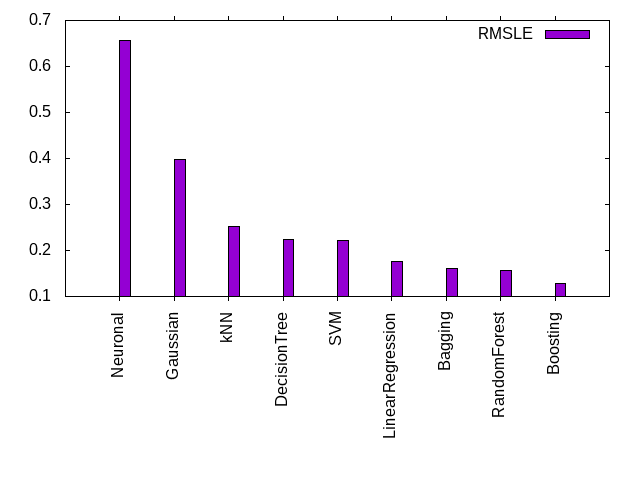
\includegraphics[scale=0.75]{./img/error.png}
	\caption{Test de algoritmos.Error.}
\end{figure}
Se puede observar que los algoritmos que mayor precisión proporcionan en este caso son los multiclasificadores. Por tanto, estudiaremos en profundidad RandomForest y Boosting para mejorar los resultados.
 \section{Herramientas.}
 Otra decisión que debemos de tomar es qué herramientas usar para abordar la resolución del problema. En primer lugar debemos elegir un lenguaje de programación, para tomar esta decisión veremos el rendimiento de algunos de los lenguajes mas usados en data mining(\url{https://www.ibm.com/developerworks/community/blogs/jfp/entry/What_Language_Is_Best_For_Machine_Learning_And_Data_Science?lang=en}). En cada caso usaremos bibliotecas open source(sklearn,weka y librerías de R). Para determinar cual de las 3 es la más conveniente en este caso, realizaré pruebas con los diferentes algoritmos y compararemos el tiempo de ejecución y el uso de memoria. Además, se debe tener en cuenta la facilidad para tratar los datos tanto para su lectura, como para la generación de los archivos con las predicciones. 
 
 Los resultados obtenidos se muestran en las siguientes gráficas:	
 \begin{figure}[!h]
 	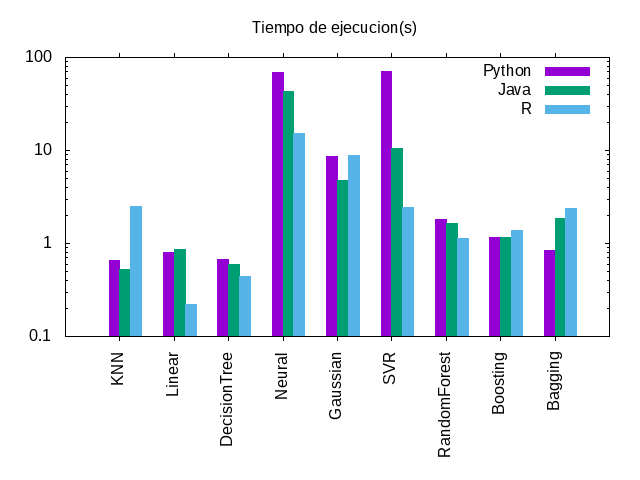
\includegraphics[scale=0.75]{./img/tiempos.png}
 	\caption{Test de algoritmos.Tiempo de ejecución}
 \end{figure}
 \begin{figure}[H]
 	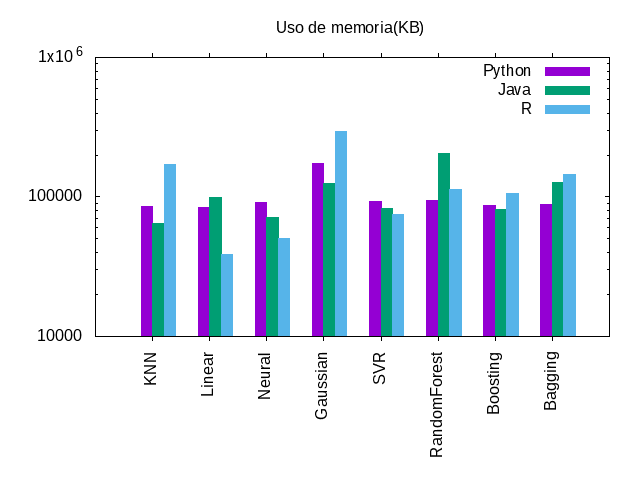
\includegraphics[scale=0.75]{./img/memoria.png}
 	\caption{Test de algoritmos.Memoria usada}
 \end{figure}
 De los resultados se deduce que no existe una alternativa que nos proporcione un rendimiento claramente superior al resto. 
 En conclusión, el lenguaje a usar será Python ya que permite un manejo de los datos flexible y un código legible propio de este lenguaje. Esta decisión se apoya en que en términos de rendimiento no hay una alternativa "mucho mejor". 
\section{Preprocesamiento}
En primer lugar elimino los outliers.Pruebo varios valores de contaminacion y me quedo el optimo.Normalizar datos. Cambiar datos missing por None(se puede entender que NaN quiere decir que no hay?)